\documentclass[12pt,a4paper,ngerman]{article}
\usepackage{stylesheet}
\usepackage{epstopdf}
\begin{document}

\TUHeader                          %  Bitte Ausfüllen!!!
%----------------------------
{Übung F: Übertragungsverhalten nachrichtentechnischer Systeme}                       %  Übungstitel
%----------------------------
{25.11.2014}                        %  Übungsdatum
%----------------------------
{05}                            %  Gruppen-Nr.
%----------------------------
{Thomas Neff}                   % Name des Protokollführers
%----------------------------
{
1.~Daniel Freßl, 1230028\\
2.~Thomas Neff, 1230319\\                    %  Übungsteilnehmer
3.~Thomas Pichler, 1230320 \\                   %  ...bei <4 Teilnehmer auskommentieren
4.~Martin Winter, 1130688\\
5.~Bernadette Schreyer, 1073076\\
}
%----------------------------
{Ao.Univ.-Prof. Dipl.-Ing. Dr. techn. Erich Leitgeb}
{Max Henkel}                          %  Betreuer
%----------------------------
{Graz}                              %  Ort der Protokollerstellung
{\today}                            %  Datum Protokollerstellung




\pagebreak
  
\tableofcontents
  
\pagebreak

%-------------------------------------------------------------------------------
%
% Beginn des Protokolls
%
%-------------------------------------------------------------------------------

\section{Analyse eines unbekannten Filters}
\subsection{Aufgabenstellung}
In dieser Aufgabe soll das Verhalten eines unbekannten Filters untersucht werden. Zuerst soll eine grundsätzliche Aussage über die Art und Ordnung des Filters getroffen und danach das Filter so eingestellt werden, dass am Ausgang maximales Überschwingen beobachtet werden kann. 
Die Eigenfrequenz dieser Konfiguration ist zu bestimmen. Weiters soll ein Bodediagramm bei einer Einstellung mit 60\% Überschwingen aufgenommen und das System durch einen äquivalenten RLC-Serienschwingkreis ersetzt werden. Dazu wird der Widerstand gemessen und L, C berechnet.

\subsection{Messaufbau}

Das unbekannte System wurde mit Hilfe eines Frequenzgenerators gespeist und die folgenden Messungen mit Hilfe eines analogen Oszilloskops gemessen. 

\subsection{Tabellen}
\begin{table}[H]
\begin{center}
\begin{tabular}{ |c|c||c|c||c|c| }
  \hline
    $\frac{T}{2}$ & $\frac{T}{2}$ & $\delta$t & $\delta$t & $U_a$ & $U_a$\\

    [$\frac{ms}{Div}$] & [Div] & [$\frac{ms}{Div}$] & [Div] & [$\frac{V}{Div}$] & [Div]\\
  \hline
$5$ & $4.6$ & $0.5$ & $0.7$ & $0.5$ & $4.0$ \\
  \hline
$0.5$ & $5.8$ & $0.5$ & $0.4$ & $0.5$ & $5.0$ \\
  \hline
$0.2$ & $6.8$ & $0.2$ & $3.4$ & $1.0$ & $6.0$ \\
  \hline
$0.2$ & $5.0$ & $0.2$ & $4.2$ & $0.5$ & $4.1$ \\
  \hline
$0.1$ & $5.0$ & $0.1$ & $4.7$ & $0.05$ & $6.4$ \\
  \hline
\end{tabular}
\caption{Gemessene halbe Periodendauer, Phasenverschiebung und Ausgangsspannung bei verschiedenen Frequenzen.}
\end{center}
\label{tab:1}
\end{table}

\begin{table}[H]
\begin{center}
\begin{tabular}{ |c|c|c|c|c|c|c| }
  \hline
    T & $\delta$t & $U_a$ & f & $\phi$ & A & $A_{dB}$\\

    [ms] & [ms] & [V] & [Hz] & [$^\circ$] & & [dB]\\
  \hline
$46$ & $0.35$ & $2$ & $21.74$ & $-2.74$ & $1$ & $0$\\
  \hline
$5.8$ & $0.2$ & $2.5$ & $172.41$ & $-12.4$ & $1.25$ & $1.94$\\
  \hline
$2.72$ & $0.68$ & $6$ & $367.65$ & $-90$ & $3$ & $9.54$\\
  \hline
$2$ & $0.84$ & $2.05$ & $500$ & $-151.2$ & $1.025$ & $0.21$\\
  \hline
$1$ & $0.47$ & $0.32$ & $1000$ & $-169.2$ & $0.16$ & $-15.92$\\
  \hline
\end{tabular}
\caption{Berechnete Periodendauer, Phasenverschiebung in ms und Grad, Ausgangsspannung, Frequenz und Verstärkung.}
\end{center}
\label{tab:1_ber}
\end{table}

\subsection{Formeln}

\subsection{Berechnungsbeispiele}

\subsection{Diagramme}
\begin{figure}[H]
\centering
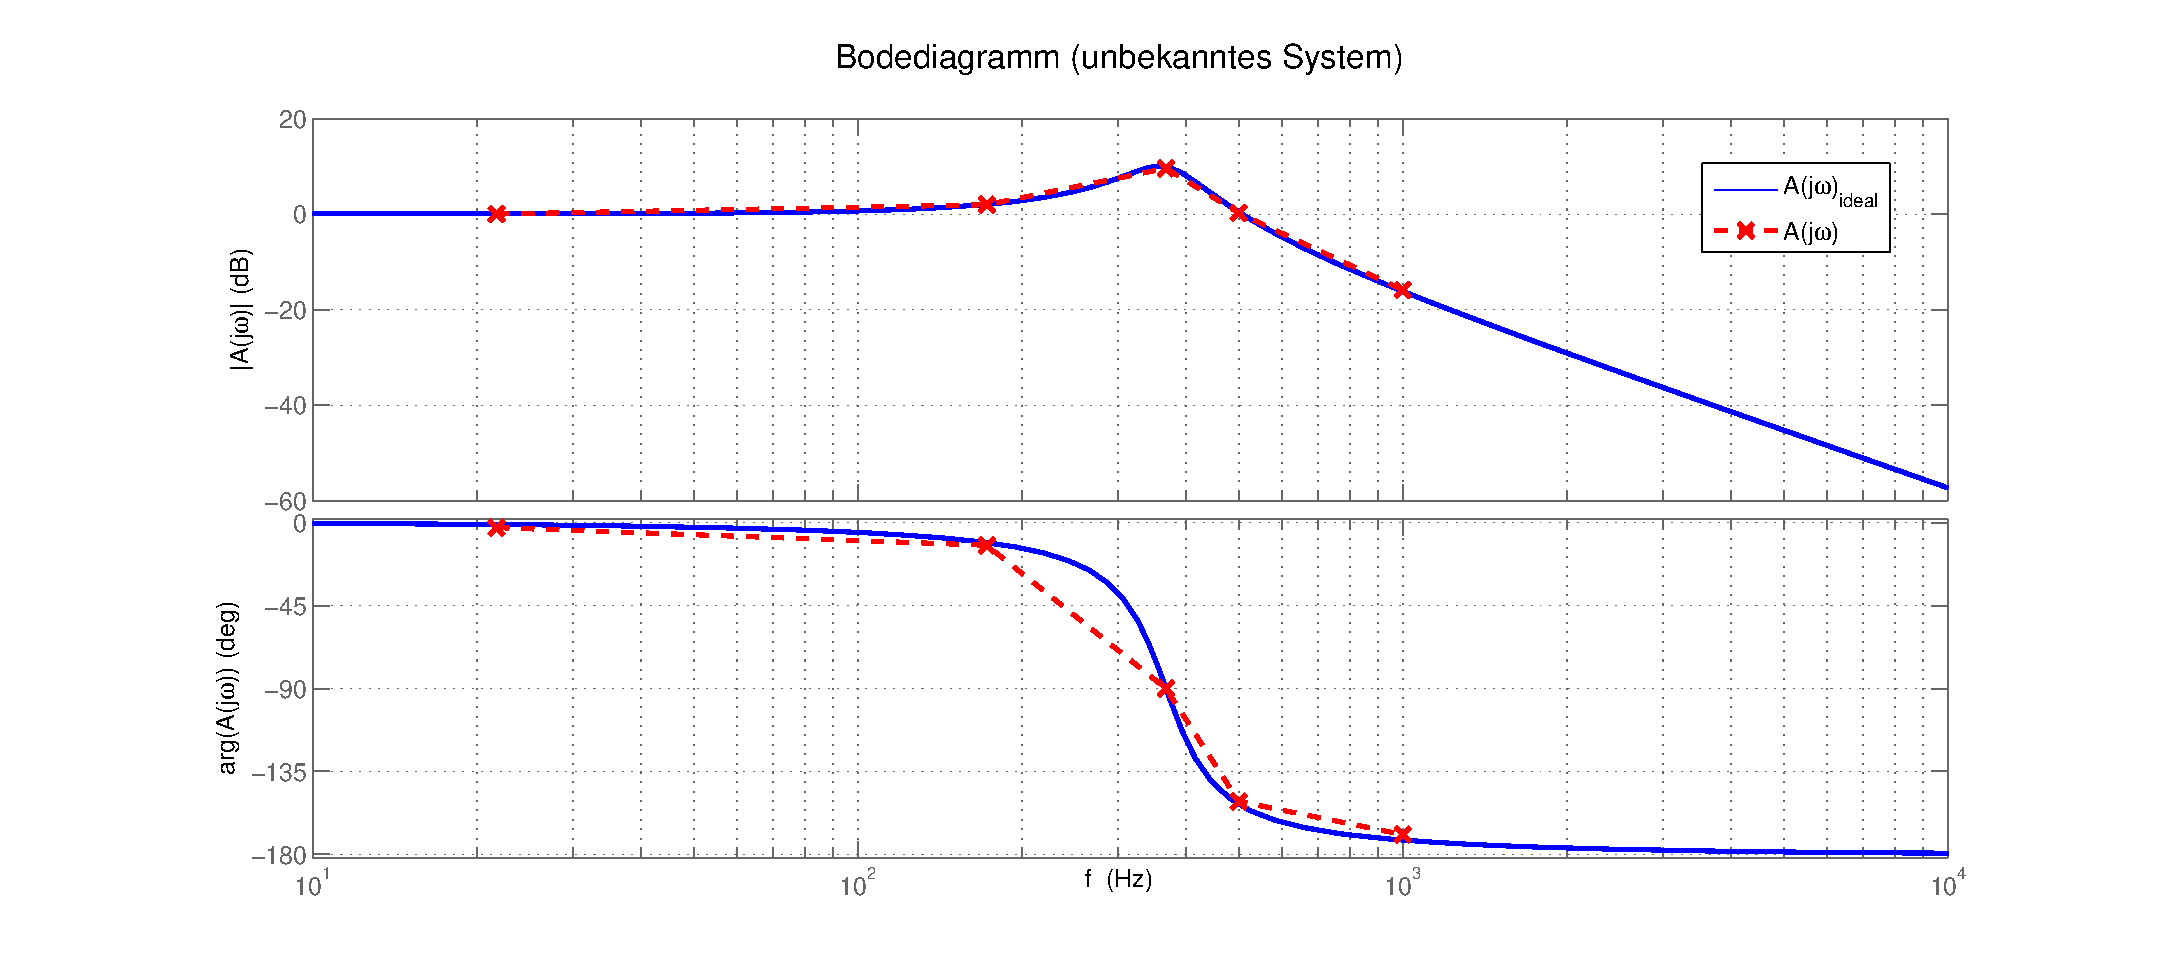
\includegraphics[width=1.2\textwidth]{figures/bode_unbekannt.eps} 
\caption{Bodediagramm des unbekannten Filters mit idealer und gemessener Kennlinie.}
\label{fig:bode_unb}
\end{figure}


\subsection{Geräteliste}
Neben dem AMREL FG-513 Funktionsgenerator und dem Voltcraft 662 Oscilloskop wurde auch ein Techtron DT-20 Multimeter verwendet.
\subsection{Diskussion}

Zunächst wurde mit Hilfe des Funktionsgenerators die Ausgangsspannung bei verschiedenen Frequenzen beobachtet. Hierbei konnten wir erkennen, dass die Phasenverschiebung bei zunehmender Frequenz stieg und die Amplitude sank. Das die Phasenverschiebung bei 3kHz $-180$ erreichte und sich ein Tiefpassverhalten ablesen ließ, muss es sich um eine Tiefpass 2. Ordnung gehandelt haben.
Um maximales Überschwingen zu erreichen, wurde ein Rechtecksignal mit kleiner Frequenz verwendet. bei einer Frequenz von $5.6$Hz und einer abgelesenen Periodendauer von $2.72$ms haben wir eine Frequenz von $367.647$Hz errechnet. Diese wurde für die weiteren Schritte als die ungedämpfte Eigenfrequenz angenommen. 
Im letzten Schritt wurden erklärt das das System durch die in Formal BLA gegebene Übertragungsfunktion beschrieben werden kann. Hierfür wurden die Bauteilwerte berechnet und in den Bodeplot eingetragen. Wie aus Diagramm BLA zu entnehmen ist, liegen die von uns gemessenen Werte sehr gut auf der idealen Kurve.



\pagebreak
\section{Analyse eines RC-Tiefpass-Filters}
\subsection{Aufgabenstellung}
Für einen RC-Tiefpass Filter mit den gegebenen Bauteilwerten $R = 13k\Omega$ und $C = 100 nF$ soll die Grenzfrequenz berechnet und gemessen werden, sowie das Bodediagramm aufgenommen werden.

\subsection{Messaufbau}
Das bekannte System wurde mit Hilfe eines Frequenzgenerators gespeist und die Eigenschaften mit Hilfe eines analogen Oszilloskops gemessen.

\subsection{Tabellen}
\begin{table}[H]
\begin{center}
\begin{tabular}{ |c|c||c|c||c|c| }
  \hline
    $\frac{T}{2}$ & $\frac{T}{2}$ & $\delta$t & $\delta$t & $U_a$ & $U_a$\\

    [$\frac{ms}{Div}$] & [Div] & [$\frac{ms}{Div}$] & [Div] & [$\frac{V}{Div}$] & [Div]\\
  \hline
$2.0$ & $5.0$ & $2.0$ & $0.6$ & $0.5$ & $4.4$ \\
  \hline
$0.5$ & $9.1$ & $0.5$ & $2.3$ & $0.5$ & $3.6$ \\
  \hline
$0.5$ & $7.6$ & $0.5$ & $2.1$ & $0.2$ & $8.2$ \\
  \hline
$0.2$ & $4.7$ & $0.2$ & $2.0$ & $0.1$ & $5.0$ \\
  \hline
$0.02$ & $4.4$ & $0.02$ & $2.0$ & $0.01$ & $4.8$ \\
  \hline
$0.001$ & $4.7$ & $0.002$ & $1.1$ & $0.001$ & $2.8$ \\
  \hline
\end{tabular}
\caption{Gemessene halbe Periodendauer, Phasenverschiebung und Ausgangsspannung bei verschiedenen Frequenzen.}
\end{center}
\label{tab:2}
\end{table}

\begin{table}[H]
\begin{center}
\begin{tabular}{ |c|c|c|c|c|c|c| }
  \hline
    T & $\delta$t & $U_a$ & f & $\phi$ & A & $A_{dB}$\\

    [ms] & [ms] & [V] & [Hz] & [$^\circ$] & & [dB]\\
  \hline
$20$ & $1.2$ & $2.2$ & $50$ & $-21.6$ & $1.1$ & $0.8$\\
  \hline
$9.1$ & $1.15$ & $1.8$ & $109.9$ & $-45.5$ & $0.9$ & $-0.92$\\
  \hline
$7.6$ & $1.05$ & $1.64$ & $131.58$ & $-49.7$ & $0.82$ & $-1.72$\\
  \hline
$1.88$ & $0.4$ & $0.5$ & $531.91$ & $-76.6$ & $0.25$ & $-12.04$\\
  \hline
$0.176$ & $0.04$ & $0.048$ & $5681.8$ & $-81.8$ & $0.024$ & $-32.4$\\
  \hline
$0.0094$ & $0.0022$ & $0.0028$ & $106382.9$ & $-84.3$ & $0.0014$ & $-57.1$\\
  \hline
\end{tabular}
\caption{Berechnete Periodendauer, Phasenverschiebung in ms und Grad, Ausgangsspannung, Frequenz und Verstärkung.}
\end{center}
\label{tab:2_ber}
\end{table}

\subsection{Formeln}

\subsection{Berechnungsbeispiele}

\subsection{Diagramme}
\begin{figure}[H]
\centering
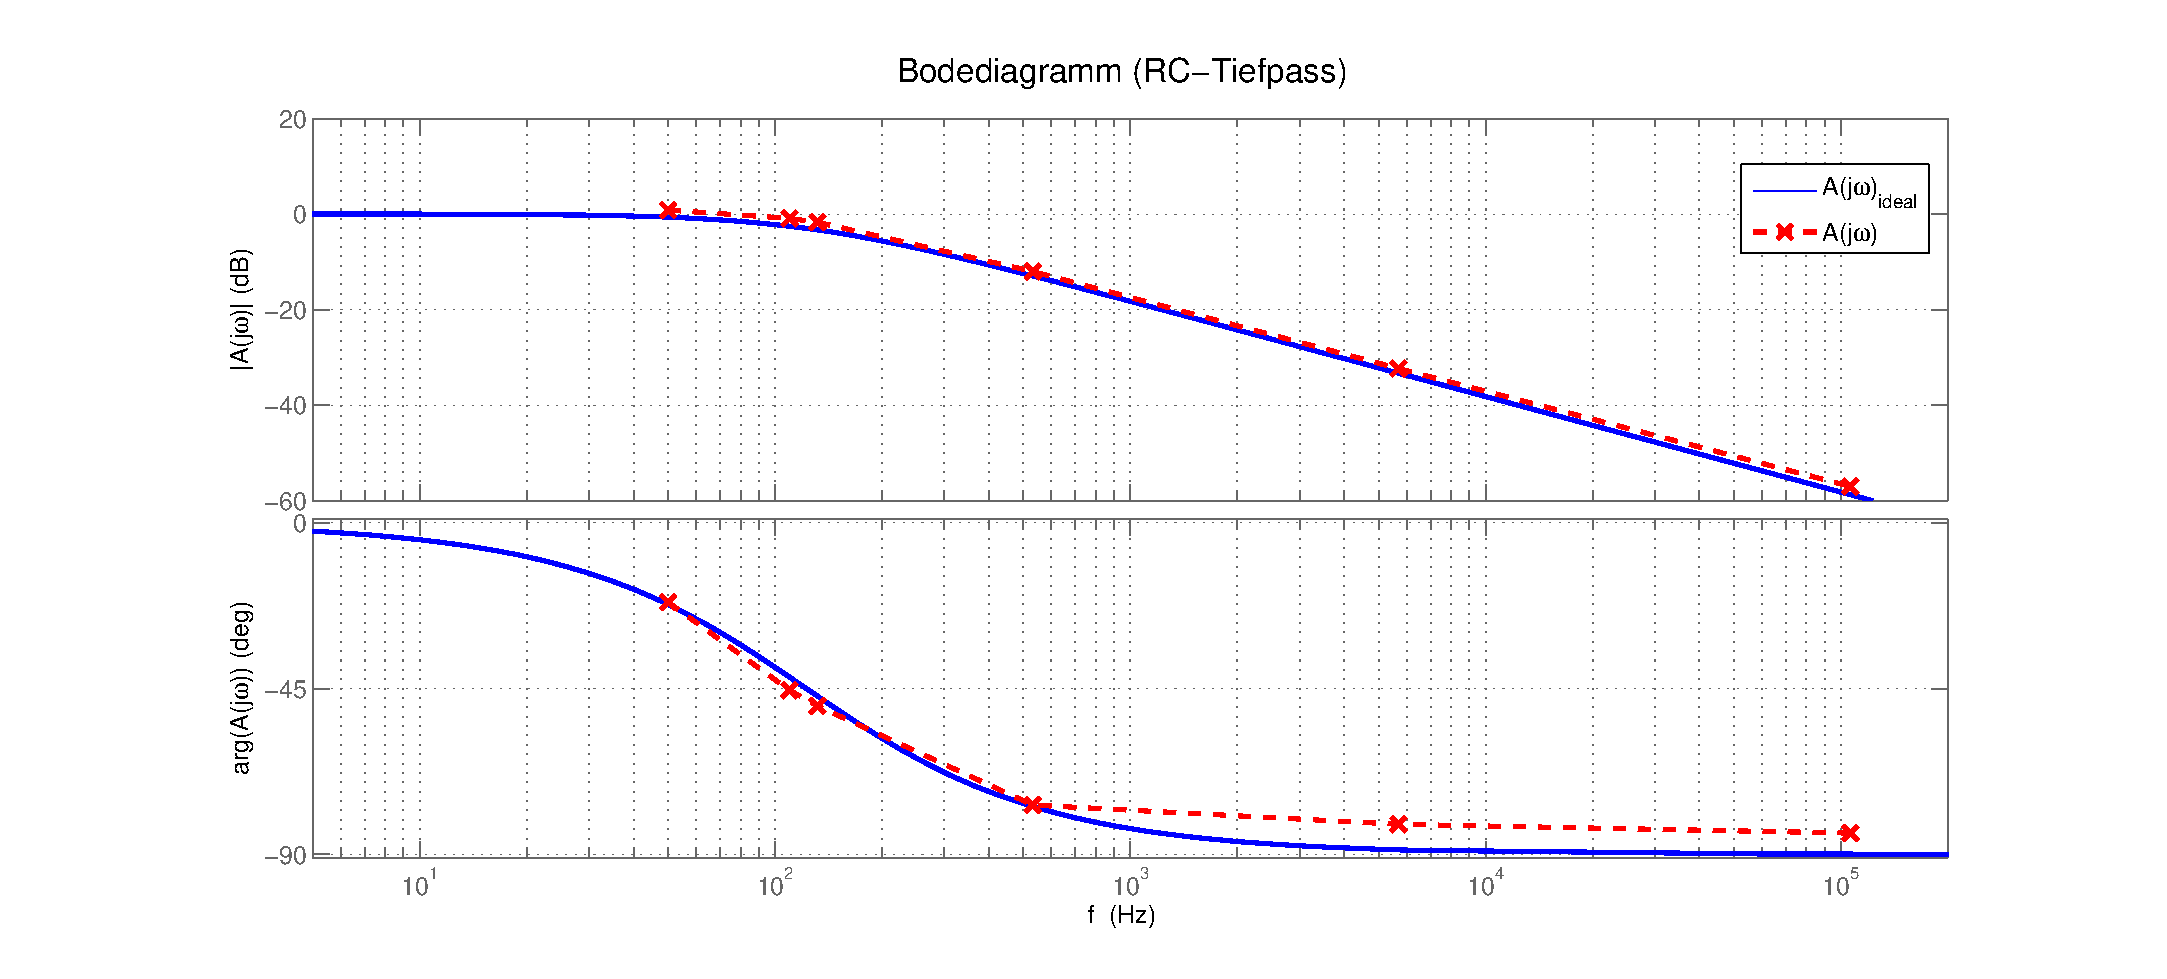
\includegraphics[width=1.1\textwidth]{figures/bode_rc.eps} 
\caption{Bodediagramm des bekannten RC-Tiefpass Filters mit idealer und gemessener Kennlinie.}
\label{fig:bode_bek}
\end{figure}


\subsection{Geräteliste}
Hier wurde wieder der AMREL FG-513 Funktionsgenerator und das Voltcraft 662 Oscilloskop verwendet.

\subsection{Diskussion}
In dieser Teilübung wurde das Bodediagramm eines bekannten Systems aufgenommen. Hierfür wurde die Phasenverschiebung und der Amplitudengang bei verschiedenen Frequenzen aufgenommen. 

%\begin{thebibliography}{9}

%\bibitem{skript}
 % Teresa Meier, Dipl.-Ing. Georg Egger, Dipl.-Ing. Dr Michael Gebhart\\
 % \emph{Übung C: RFID}\\
 % Technische Universität Graz
%\end{thebibliography}

 



   
\end{document}
